\documentclass{article} % Definisi jenis dokumen

%%%%% Definisi paket-paket yang seharusnya digunakan %%%%%
\usepackage[utf8]{inputenc} % paket encoding input utf8
\usepackage[T1]{fontenc} % paket encoding huruf latin

%%%%% Definisi paket-paket yang digunakan sesuai kebutuhan %%%%%
\usepackage[yyyymmdd,hhmmss]{datetime} % paket tanggal-waktu
\usepackage{graphicx} % paket grafik/gambar
\usepackage[english]{babel} % paket modifikasi label/caption pada bahasa tertentu
\usepackage{geometry} % paket ukuran kertas dan margin
\usepackage{pdfpages}

%%%%% Pengaturan ukuran kertas dan margin %%%%%
\geometry{
	a4paper,
	left=10mm,
	right=10mm,
	top=15mm,
	bottom=15mm,
}

\begin{document}
	\begin{titlepage}

		\centering % untuk membuat tengah teks

		{
			\LARGE % pakai font besar
			\bf % pakai font BOLD
			Rangkuman Email Proses Impor
		}

		\bigskip
		{\Large \bf Tim Penelitian Audiometri Dhany Arifianto}
		\vfill % menambahkan ruang kosong vertikal
	\end{titlepage}

	\newpage
	\section{Deskripsi}

	Berikut kami jabarkan permasalahan impor barang penelitian kami yang masih tertahan di warehouse PT Chanda Adhi Sentosa (CAS) selaku broker PT UPS Cardig International.\\

	Perlu disampaikan bahwa:
	\begin{itemize}
		\item Tidak ada dari tim riset yang memahami proses clearance impor.
		\item Tidak ada dari tim riset yang memahami bahwa entitas ITS, ITS PTN-BH, dan Bapak Dhany Arifianto seharusnya diperlukan sebagai entitas yang berbeda dalam administrasi impor.
		\item Tidak ada dari tim riset yang memahami terkait NIB atau identitas usaha lain, yang notabene baik ITS dan Bapak Dhany Arifianto sama-sama tidak memiliki dokumen tersebut.
	\end{itemize}

	Produk yang bermasalah adalah Simulator Telinga dari vendor 3DIO yang berada di US.
	Untuk dokumen terkait telah dilampirkan pada dokumen ini.

	\section{Tabel Kronologi Proses Impor}

	\begin{table}[!ht]
		\begin{tabular}{|l|l|l|}
		\hline
		\textbf{Tanggal}	& \textbf{Deskripsi} & \textbf{Keterangan}  \\ \hline
		5 September 2022	& Barang telah sampai di Indonesia &  \\ \hline
		14 September 2022	& UPS/CAS mengontak ITS & Tidak respon oleh ITS \\ \hline
		16-23 September 2022	& UPS/CAS kembali mengontak ITS & Tidak respon oleh ITS \\ \hline
		28 September 2022	& Tim Peneliti secara mandiri mengontak UPS & Dokumen shipment kami terima \\ \hline
		28 September 2022	& Barang dikonfirmasi sebagai milik ITS &  \\ \hline
		28 September 2022	& Peneliti diminta melengkapi NPWP dan NIB milik ITS & Peneliti belum paham terkait NIB  \\ \hline
		29 September 2022	& Peneliti diminta mengurus dokumen redress ITS ke ITS PTN BH &  \\ \hline
		8 Oktober 2022	& Email shipper untuk redress telah kami terima &  \\ \hline
		13 Oktober 2022	& CAS kembali konfirmasi NIB &  ITS tidak memiliki NIB \\ \hline
		20 Oktober 2022 & Proses Redress berubah ke nama Peneliti &  \\ \hline
		21 Oktober 2022 & Peneliti perjalanan konferensi ke Korea & Pengurusan Redress tertahan  \\ \hline
		25 Oktober 2022 & CAS meminta dokumen permohonan POS BCF 1.5 & Shipment sudah lebih dari 30 hari   \\ \hline
		\end{tabular}
	\end{table}

	\newpage
	\section{Lampiran Screenshot Kronologi Email}

	\begin{itemize}
		\item Menurut Tracking UPS, barang telah sampai di Indonesia tanggal 5 September 2022

		\begin{figure}[!ht]
			\centering
			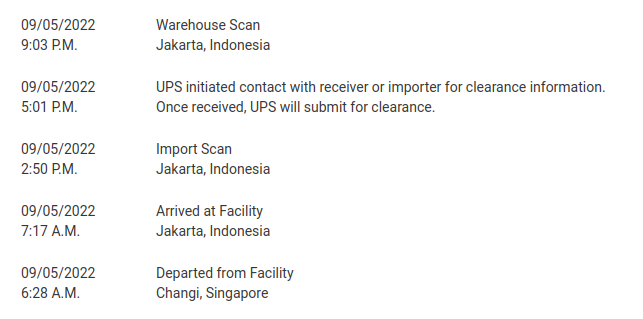
\includegraphics[width=400pt]{images/impor_0}
		\end{figure}

		\item Tanggal 14 September 2022, PT. Chandra Adi Sentosa (CAS) selaku broker PT UPS Cardig International mengontak Humas ITS via email.

		\begin{figure}[!ht]
			\centering
			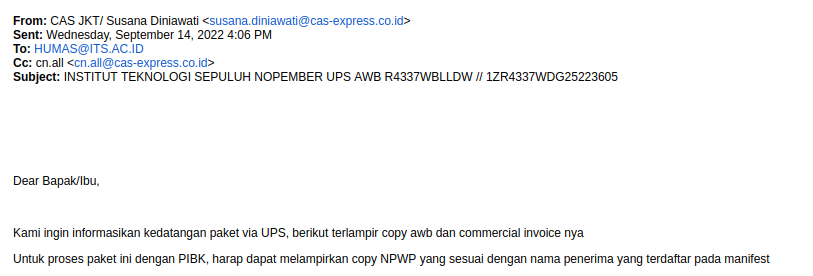
\includegraphics[width=400pt]{images/impor_1}
		\end{figure}

		Mengingat bukan pihak ITS bukan pengimpor, maka email tersebut tidak dihiraukan oleh pihak ITS dan tidak ada notifikasi ke tim peneliti

		\item Tanggal 15 September 2022, pihak CAS kembali mengontak pihak ITS dan kembali tidak dihiraukan.

		\begin{figure}[!ht]
			\centering
			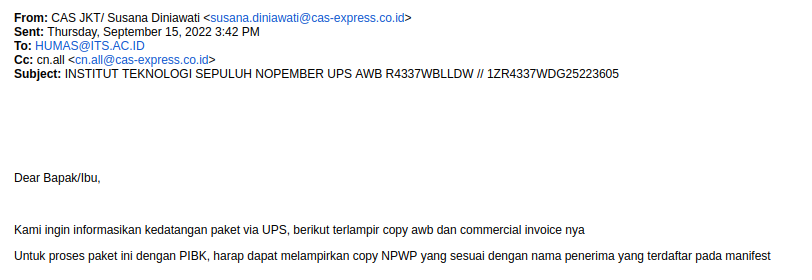
\includegraphics[width=400pt]{images/impor_2}
		\end{figure}

		Pihak CAS kembali mengontak pihak ITS dengan email sama pada tanggal 16, 19, 20, 21, 22, dan 23 di bulan September 2022

		\newpage
		\item Tanggal 28 September 2022, salah satu anggota peneliti melakukan inisitiatif tracking mandiri dan mengontak UPS secara personal.
		Anggota Peneliti tersebut kemudian mendapat email yang sama dan telah direspon.

		\begin{figure}[!ht]
			\centering
			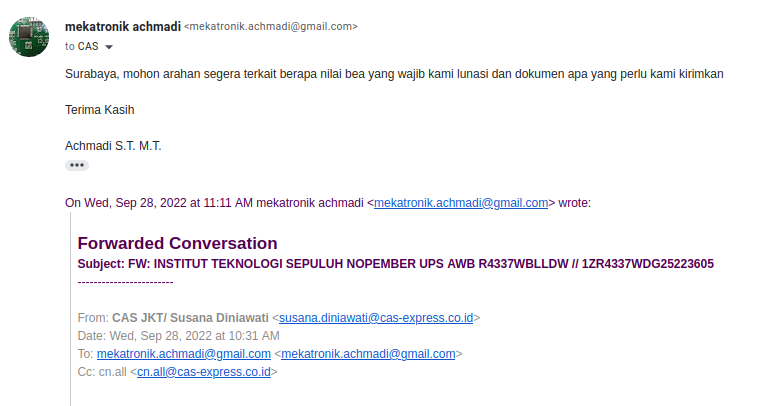
\includegraphics[width=400pt]{images/impor_3}
		\end{figure}

		Disini dokumen shipment dan notice of arrival telah diterima peneliti.

		\item Pihak CAS menanyakan konfirmasi terkait kepemilikian barang

		\begin{figure}[!ht]
			\centering
			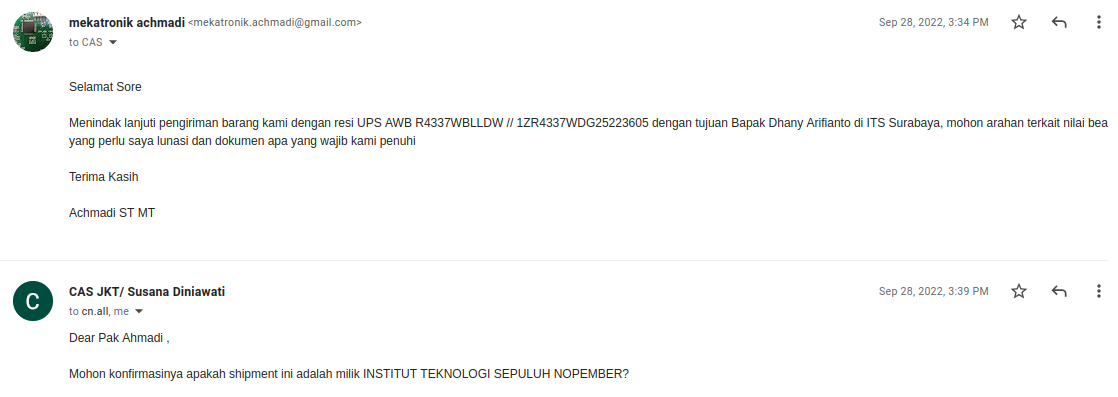
\includegraphics[width=400pt]{images/impor_4}
		\end{figure}

		Kami konfirmasi kepemilikan barang tersebut

		\begin{figure}[!ht]
			\centering
			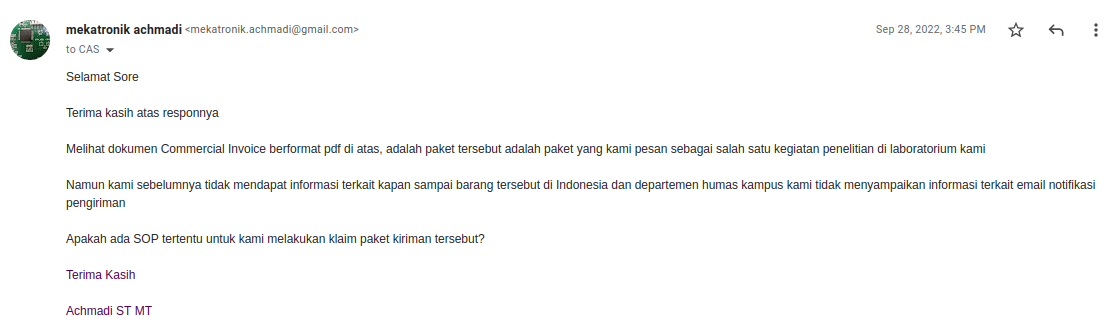
\includegraphics[width=400pt]{images/impor_5}
		\end{figure}

		\item Paket kemudian terkonfirmasi sebagai milik INSTITUT TEKNOLOGI SEPULUH NOPEMBER
		Kami diminta melampirkan NPWP dan NIB dari kampus ITS

		\begin{figure}[!ht]
			\centering
			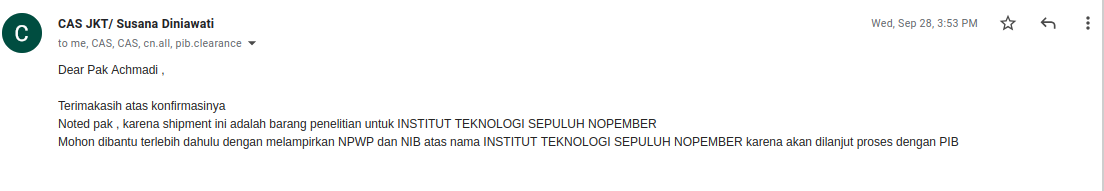
\includegraphics[width=400pt]{images/impor_6}
		\end{figure}

		\newpage
		\item Kami melampirkan NPWP dan SKT atas nama ITS PTN BH.
		Pada saat itu kami belum paham mengenai dokumen NIB.

		\begin{figure}[!ht]
			\centering
			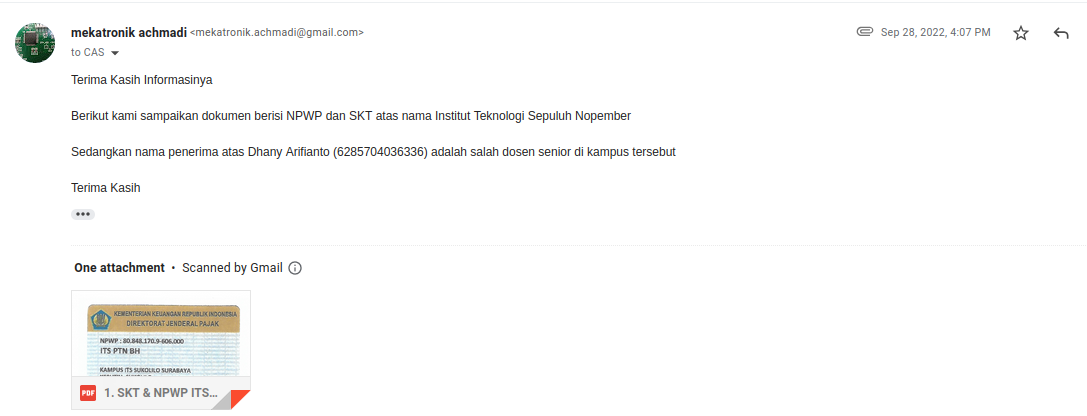
\includegraphics[width=400pt]{images/impor_7}
		\end{figure}

		\item Tanggal 29 September 2022, kami diminta melakukan redress (perubahan penerima/tujuan),
		Dikarenakan NPWP/SKT atas nama ITS PTN BH, bukan INSTITUT TEKNOLOGI SEPULUH NOPEMBER

		\begin{figure}[!ht]
			\centering
			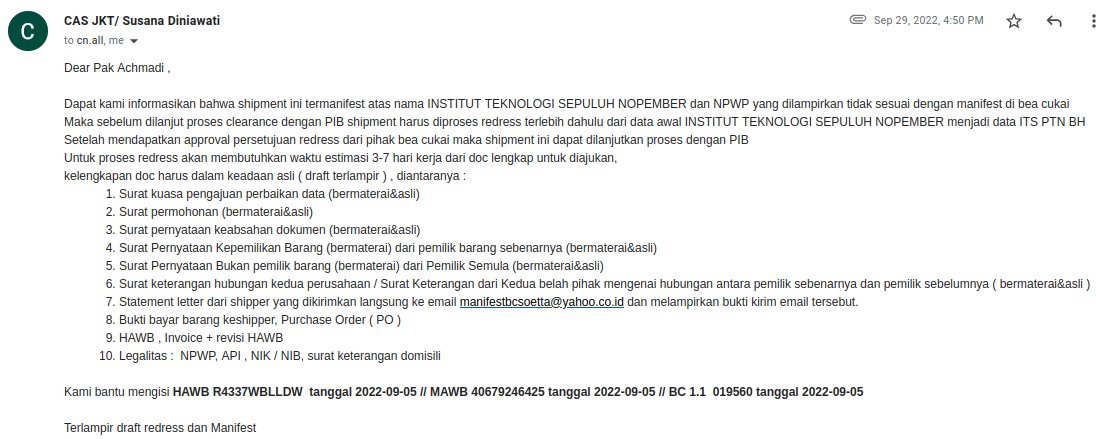
\includegraphics[width=400pt]{images/impor_8}
		\end{figure}

		\item Kami menjelaskan bahwa ITS dan ITS PTN BH adalah sama dan kami lampirkan pula screenshoot pembelian

		\begin{figure}[!ht]
			\centering
			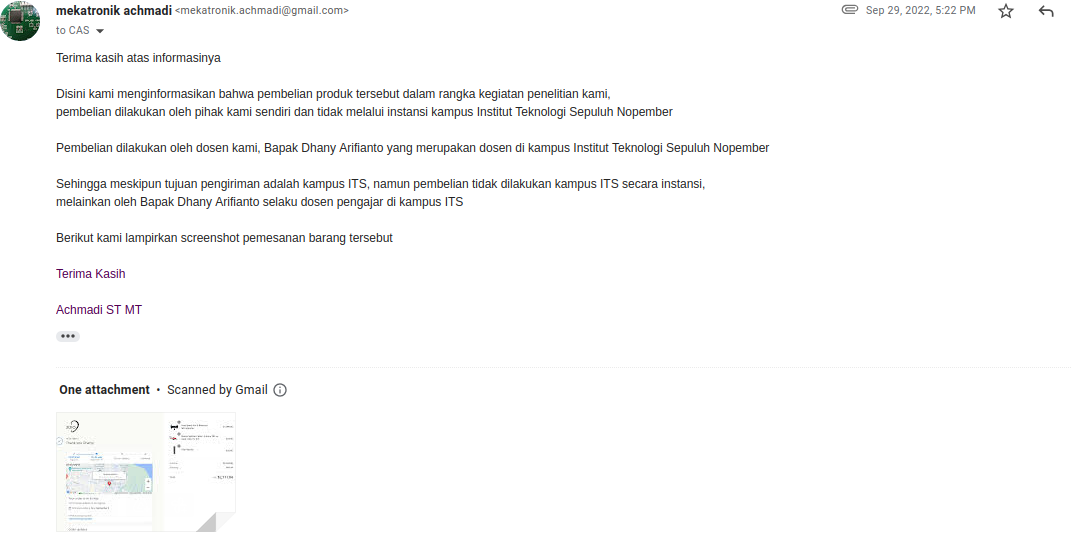
\includegraphics[width=400pt]{images/impor_9}
		\end{figure}

		\newpage
		\item Tanggal 5 Oktober 2022, kami mendapat email konfirmasi bahwa ITS dan ITS PTN BH tidak bisa disamakan terkait dokumen NPWP.

		\begin{figure}[!ht]
			\centering
			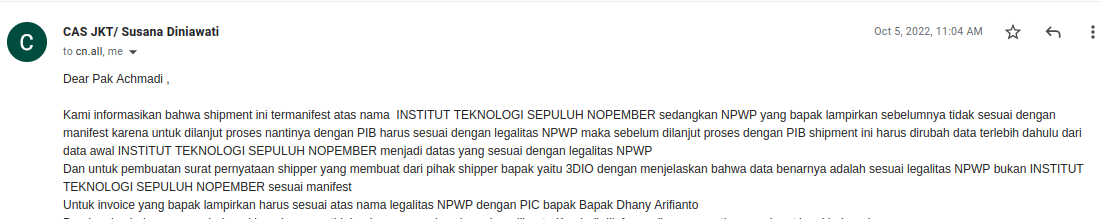
\includegraphics[width=400pt]{images/impor_10}
		\end{figure}

		Jika ingin redress ke atas nama peneliti, harus tetap melakukan proses redress

		\begin{figure}[!ht]
			\centering
			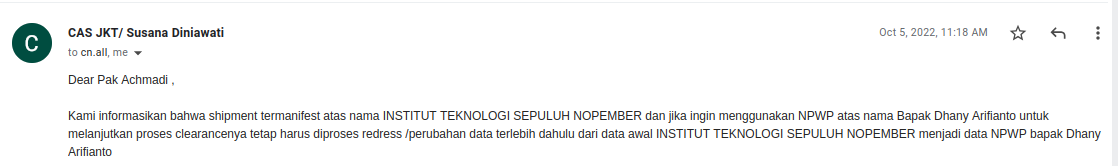
\includegraphics[width=400pt]{images/impor_11}
		\end{figure}

		\item Proses Pengurusan Redress kami laksanakan dan kami sudah mendapat email dari shipper (3DIO US) terkait redress

		\begin{figure}[!ht]
			\centering
			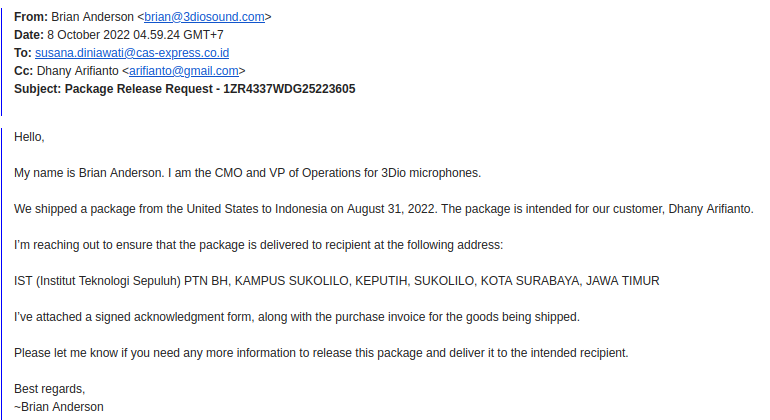
\includegraphics[width=300pt]{images/impor_12}
		\end{figure}

		Hingga mendapat email ini, dokumen redress masih belum selesai pengurusan ke pihak ITS karena banyak revisi konten dokumen.

		\item Tanggal 13 Oktober 2022, pihak CAS menanyakan mengkonfirmasi kewajiban dokumen NIB, dimana tidak dapat kami penuhi.

		\begin{figure}[!ht]
			\centering
			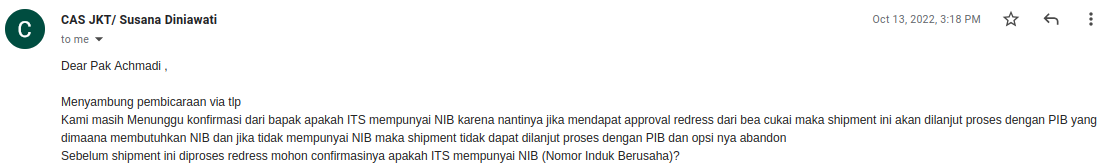
\includegraphics[width=400pt]{images/impor_13}
		\end{figure}

		\item Tanggal 20 Oktober 2022, proses redress kemudian berubah ke tujuan Bapak Dhany Arifianto

		\begin{figure}[!ht]
			\centering
			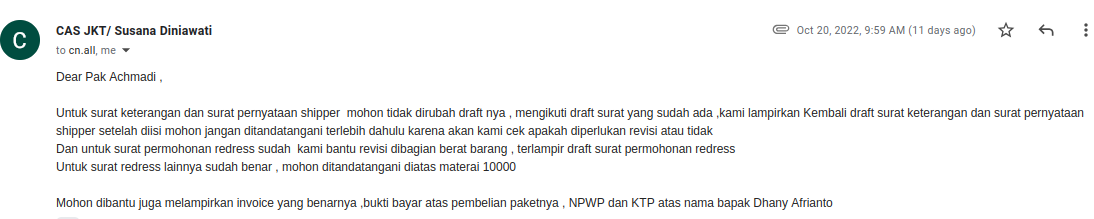
\includegraphics[width=400pt]{images/impor_14}
		\end{figure}

		\newpage
		\item Tanggal 21 Oktober 2022, Bapak Dhany Arifianto berangkat ke Korea untuk kegiatan konferensi.
		Pengurusan Dokumen Redress berhenti sementara.

		\item Tanggal 25 Oktober 2022, pihak CAS meminta dokumen POS BCF 1.5 dikarenakan shipment sudah lebih dari 30 hari.

		\begin{figure}[!ht]
			\centering
			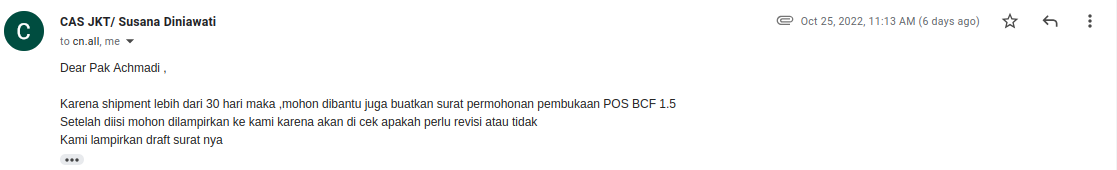
\includegraphics[width=400pt]{images/impor_15}
		\end{figure}

	\end{itemize}

	\section{Dokumen Terkait}

	\subsection{Screenshot Pembelian}

	\begin{figure}[!ht]
		\centering
		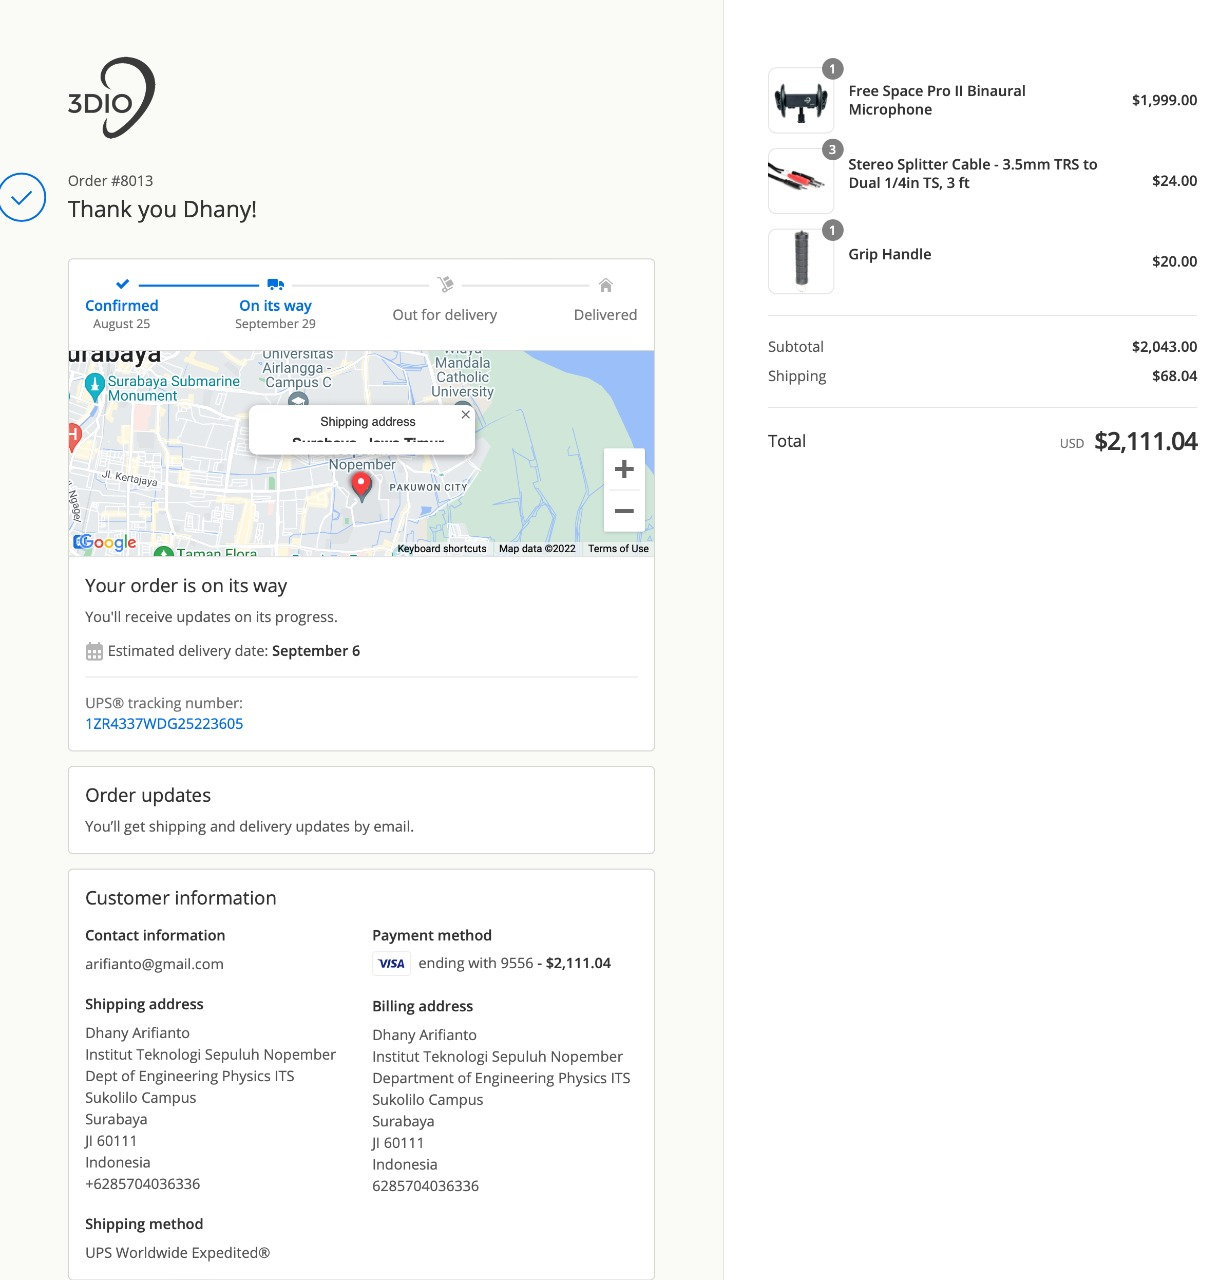
\includegraphics[width=400pt]{images/pesan3DIO}
	\end{figure}

	\subsection{Dokumen Shipment}

	Berikut dilampirkan dokumen shipment dan notice of arrival dari produk yang dibeli oleh peneliti.

	\includepdf[pages=-]{pdfs/R4337WBLLDW_NOA.pdf}
	\includepdf[pages={1}]{pdfs/R4337WBLLDW.pdf}

	\begin{figure}[!ht]
		\centering
		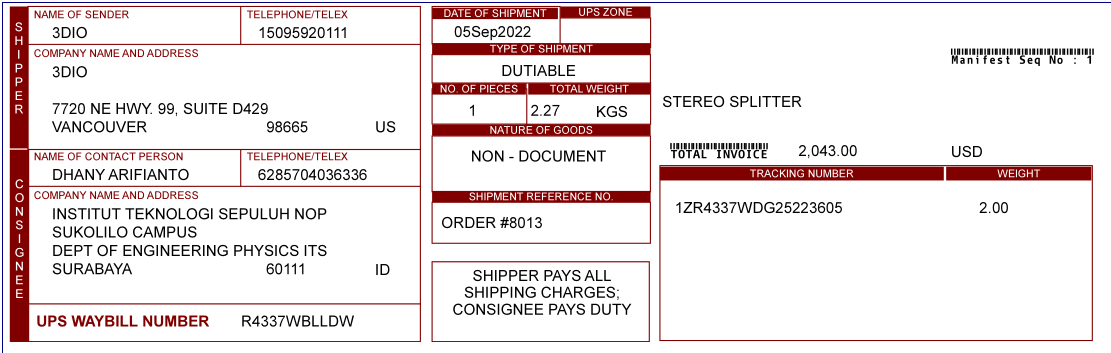
\includegraphics[width=400pt]{images/shipment}
	\end{figure}
\end{document}
